\documentclass[letterpaper,11pt]{article}
\usepackage{graphicx}
\usepackage{listings}
\usepackage[super]{nth}
\usepackage[hyphens]{url}
\usepackage{hyperref}
\usepackage{amsmath}
\usepackage[makeroom]{cancel}
\usepackage[table]{xcolor}
\usepackage{comment}
\usepackage[space]{grffile}
\usepackage{csvsimple}
\usepackage{longtable}
\usepackage{adjustbox}


\newcommand*{\srcPath}{../src}%

\lstset{
	basicstyle=\footnotesize,
	breaklines=true,
}

\begin{document}

\begin{titlepage}

\begin{center}

\Huge{Assignment 2}

\Large{CS 734:  Introduction to Information Retrieval}

\Large{Fall 2017}

\Large{Grant Atkins}

\Large Finished on \today

\end{center}

\end{titlepage}

\newpage


% =================================
% First question
% =================================
\section*{1}

\subsection*{Question}

\begin{verbatim}
4.1. Plot rank-frequency curves (using a log-log graph) for 
words and bigrams in the Wikipedia collection available through 
the book website (http://www.searchengines-book.com). Plot a 
curve for the combination of the two. What are the best 
values for the parameter c for each curve?
\end{verbatim}

\subsection*{Answer}

For this question I wrote two files of code, \textbf{rankFreq.py} and \textbf{rankFreq.R} in with the ``small'' wiki dataset provided from the textbooks website . 
The first python file iterates through all of the wiki html files, tokenizes them, finds token frequency, and then writes them to a CSV in descending frequency order.
To retrieve the text from each of the html files I used Beautifulsoup. 
It should be noted when retrieving each token from the html files I did not take into account uppercase or lowercase as same terms, I treated them as different and more than probably affected the outcome of this answer.
After the code tokenizing the terms it created a list of unigrams and bigrams for all the terms keeping them in separate lists to count frequencies.
I used the NLTK python library to make bigram pairs.
The code for this is shown below in Listing \ref{lst:q1py}.
The top 10, ranked by token frequency, results are shown below in Figures \ref{fig:q1uni} and \ref{fig:q1bi}.
The full CSV files can be found in my Github repository \cite{github}.
Without removing stop words its apparent that words like ``the'' and ``of'' would some of the top unigram and bigram pairs.

 \lstinputlisting[frame=single,caption={Python script to tokenize and find frequencies and calculate C parameters},label=lst:q1py,captionpos=b,numbers=left,showspaces=false,showstringspaces=false,basicstyle=\footnotesize]{\srcPath/rankFreq.py}
 
 To create the graphs I used R's ggplot2 library. 
 The code to create these graphs is shown in Listing \ref{lst:q1R}.
 The figures created from the afore mentioned code are shown in Figure \ref{fig:q1p1}, \ref{fig:q1p2}, and \ref{fig:q1p3}.
For unigrams the best \textit{C} parameter was 0.14, while for bigrams it was 0.1.
 
  \lstinputlisting[frame=single,caption={Python script to tokenize and find frequencies and calculate C parameters},label=lst:q1R,captionpos=b,numbers=left,showspaces=false,showstringspaces=false,basicstyle=\footnotesize]{\srcPath/rankFreq.R}

  \begin{figure}[h]
  \centering
  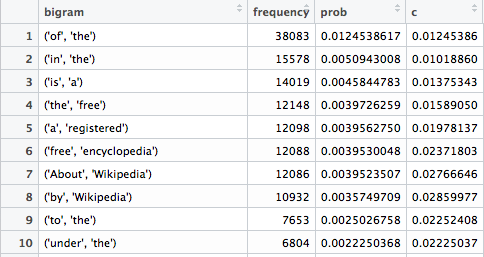
\includegraphics[scale=0.6]{unigram_10.png}
  \caption{Top 10 unigrams found}
  \label{fig:q1uni}
  \end{figure}

  \begin{figure}[h]
  \centering
  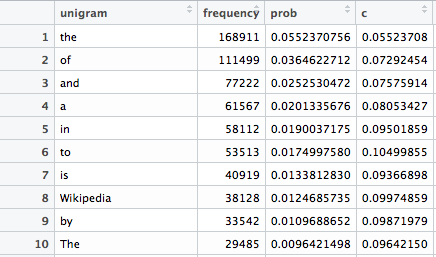
\includegraphics[scale=0.6]{bigram_10.png}
  \caption{Top 10 bigrams found}
  \label{fig:q1bi}
  \end{figure}
  
   \begin{figure}[h]
  \centering
  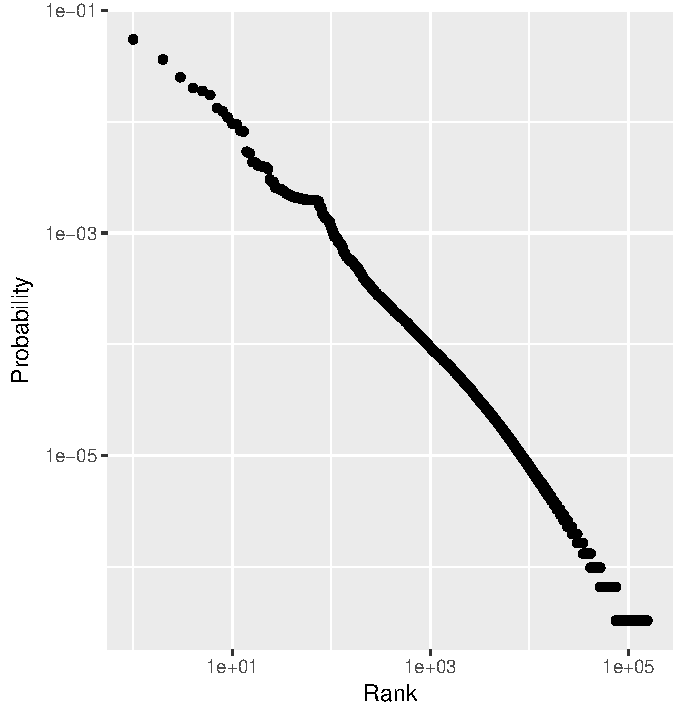
\includegraphics[scale=0.6]{unigram_plot.pdf}
  \caption{Log-log plot of unigram frequency and probability}
  \label{fig:q1p1}
  \end{figure}

   \begin{figure}[h]
  \centering
  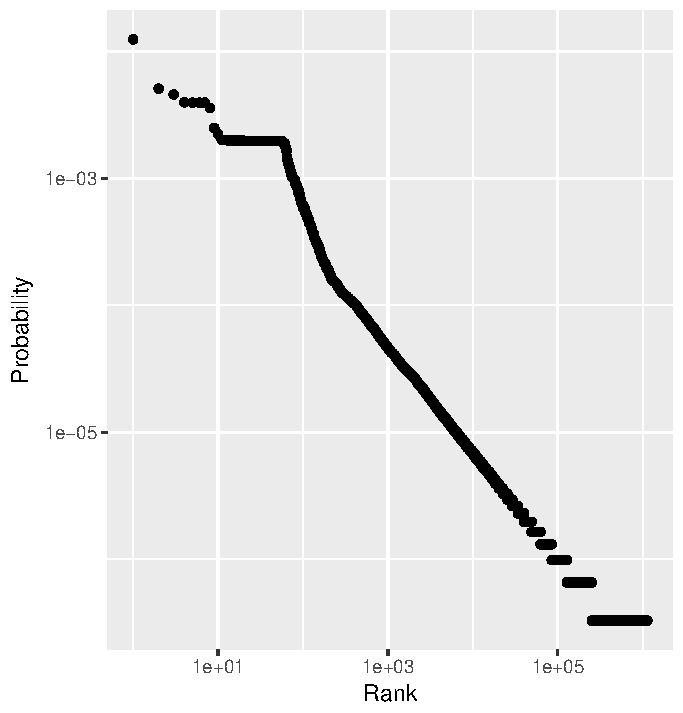
\includegraphics[scale=0.6]{bigram.pdf}
  \caption{Log-log plot of bigram frequency and probability}
  \label{fig:q1p2}
  \end{figure}
  
   \begin{figure}[h]
  \centering
  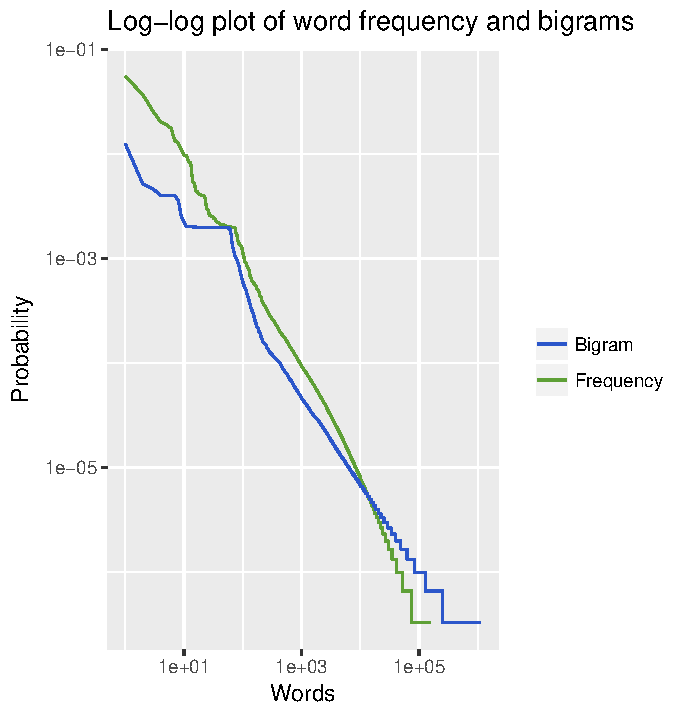
\includegraphics[scale=0.9]{unigram_and_bigram.pdf}
  \caption{Log-log plot of unigram and bigram frequencies and probabilities}
  \label{fig:q1p3}
  \end{figure}


\clearpage

% =================================
% Second question
% =================================

\section*{2}

\subsection*{Question}

\begin{verbatim}
4.2. Plot vocabulary growth for the Wikipedia collection and estimate 
the parameters for Heaps' law. Should the order in which the 
documents are processed make any difference?
\end{verbatim}

\subsection*{Answer}

To answer this question I again created two files, \textbf{vocabGrowth.py} and \textbf{vocabGrowth.R}.
My python script use the Beautifulsoup library to parse out the html documents of the small wikipedia example.
Much like my answer to the first question I traversed the html documents in order and then in reverse, each time tokenizing the text of html, taking an overall corpus count, and tracking unique vocabulary through each of the html documents. 
The code for this is shown in Listing \ref{lst:q2py}.
The goal of this was simply see how the unique vocabulary list grows while the corpus size continues to grow.

  \lstinputlisting[frame=single,caption={Python script to tokenize and find frequencies and calculate C parameters},label=lst:q2py,captionpos=b,numbers=left,showspaces=false,showstringspaces=false,basicstyle=\footnotesize]{\srcPath/vocabGrowth.R}

The relationship between corpus size and vocabulary size was defined in our book as: \[ v = k * n^\beta \].

To estimate the parameters for heaps law and plot the vocabulary growth, I used R's ggplot2 to create charts and the built in function non-linear least squares (nls).
The parameters of K and B were initialized with a value of one. 
The plot of documents traversed in order is shown in Figure \ref{fig:q2p1} and the plot of the documents traversed in reverse is shown in Figure \ref{fig:q2p2}.
The plots show vocab count along the y-axis and corpus word count along x-axis.
It is apparent that these two graphs are different and that means the order in which the documents are processed does make a difference.

The estimation parameters for Heap's law for in order and reverse, computed by the nls method in R, are shown in Table \ref{table:heap}. 
Some of values do differ slightly, such as the B values for ascending and descending, but there is an apparent difference which further supporting my claim.

\begin{table}
\centering
\begin{tabular}{|l|l|l|}
\hline
\multicolumn{1}{|c|}{\textbf{Number}} & \multicolumn{1}{c|}{\textbf{Parameter}} & \multicolumn{1}{c|}{\textbf{Values}} \\ \hline
1 & Document Count & 6043 \\ \hline
2 & K ascending & 7.6679986 \\ \hline
3 & B ascending & 0.6652129 \\ \hline
4 & K descending & 6.276427 \\ \hline
5 & B descending & 0.678342 \\ \hline
\end{tabular}
\caption{Heap's Law parameters for Small Wiki}
\label{table:heap}
\end{table}

   \begin{figure}[h]
  \centering
  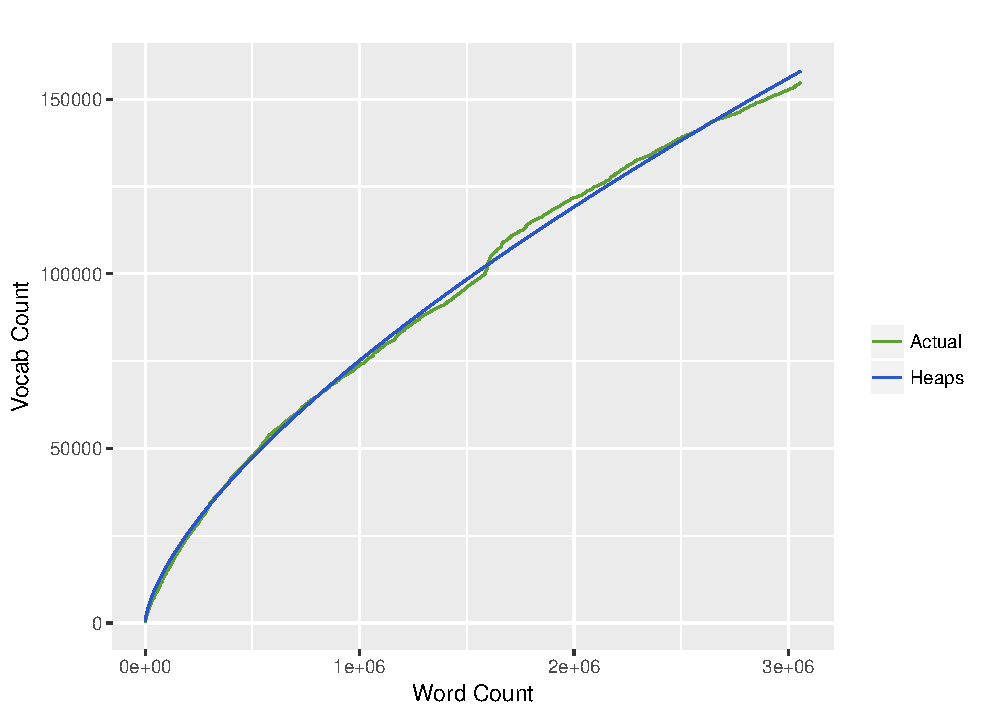
\includegraphics[scale=0.7]{corpusGrowth.pdf}
  \caption{Growth of vocabulary vs overall corpus}
  \label{fig:q2p1}
  \end{figure}
  
   \begin{figure}[h]
  \centering
  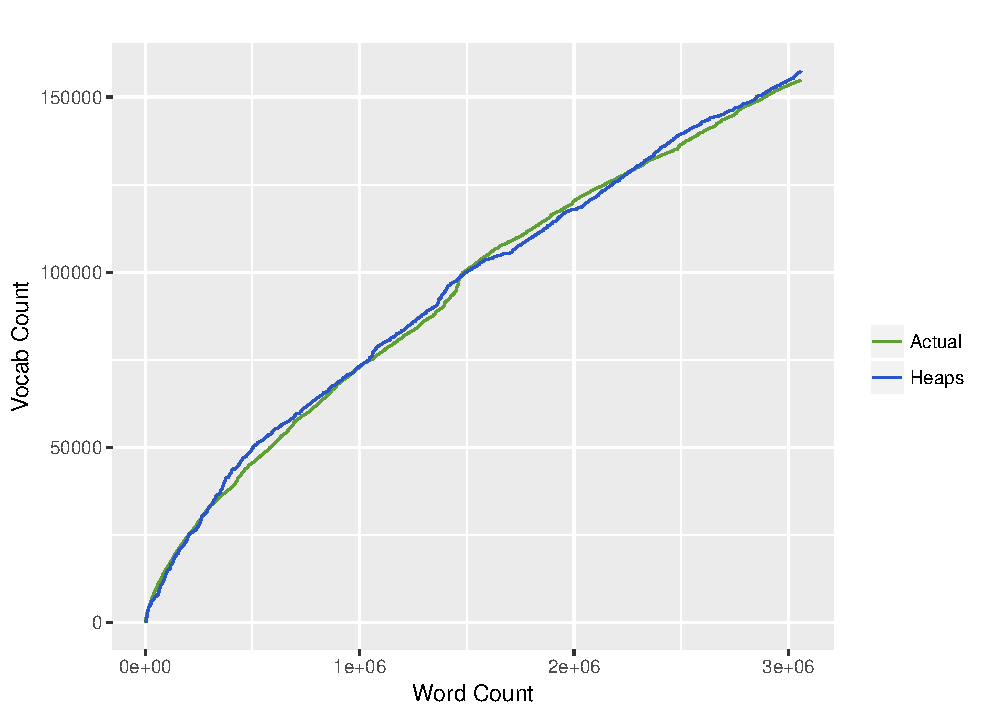
\includegraphics[scale=0.7]{corpusGrowthReverse.pdf}
  \caption{Growth of vocabulary vs overall corpus with documents traversed in reverse}
  \label{fig:q2p2}
  \end{figure}

\clearpage

% =================================
% 3rd question
% =================================

\section*{3}

\subsection*{Question}

\begin{verbatim}

\end{verbatim}

\subsection*{Answer}



\clearpage

% =================================
% 4th question
% =================================

\section*{4}

\subsection*{Question}

\begin{verbatim}

\end{verbatim}

\subsection*{Answer}


\clearpage

% =================================
% 5th question
% =================================

\section*{5}

\subsection*{Question}

\begin{verbatim}

\end{verbatim}

\subsection*{Answer}


\clearpage


% =================================
% Bibliography
% =================================

\begin{thebibliography}{9}
\bibitem{cs532}
Atkins, Grant. ``CS532 Assignment 1 Repository'' Github. N.p., 23 March 2017. Web. 23 March 2017.\url{https://github.com/grantat/cs532-s17/tree/master/assignments/A1/src}.
\bibitem{github}
Atkins, Grant. ``CS734 Assignment 2 Repository'' Github. N.p., 21 September 2017. Web. 21 September 2017.\url{https://github.com/grantat/cs834-f17/tree/master/assignments/A2}.
\end{thebibliography}

\end{document}
